% !TeX program = pdfLaTeX
\documentclass[12pt]{article}
\usepackage{amsmath}
\usepackage{graphicx,psfrag,epsf}
\usepackage{enumerate}
\usepackage{natbib}
\usepackage{textcomp}
\usepackage[hyphens]{url} % not crucial - just used below for the URL
\usepackage{hyperref}
\providecommand{\tightlist}{%
  \setlength{\itemsep}{0pt}\setlength{\parskip}{0pt}}

%\pdfminorversion=4
% NOTE: To produce blinded version, replace "0" with "1" below.
\newcommand{\blind}{0}

% DON'T change margins - should be 1 inch all around.
\addtolength{\oddsidemargin}{-.5in}%
\addtolength{\evensidemargin}{-.5in}%
\addtolength{\textwidth}{1in}%
\addtolength{\textheight}{1.3in}%
\addtolength{\topmargin}{-.8in}%

%% load any required packages here


\usepackage{color}
\usepackage{fancyvrb}
\newcommand{\VerbBar}{|}
\newcommand{\VERB}{\Verb[commandchars=\\\{\}]}
\DefineVerbatimEnvironment{Highlighting}{Verbatim}{commandchars=\\\{\}}
% Add ',fontsize=\small' for more characters per line
\usepackage{framed}
\definecolor{shadecolor}{RGB}{248,248,248}
\newenvironment{Shaded}{\begin{snugshade}}{\end{snugshade}}
\newcommand{\AlertTok}[1]{\textcolor[rgb]{0.94,0.16,0.16}{#1}}
\newcommand{\AnnotationTok}[1]{\textcolor[rgb]{0.56,0.35,0.01}{\textbf{\textit{#1}}}}
\newcommand{\AttributeTok}[1]{\textcolor[rgb]{0.77,0.63,0.00}{#1}}
\newcommand{\BaseNTok}[1]{\textcolor[rgb]{0.00,0.00,0.81}{#1}}
\newcommand{\BuiltInTok}[1]{#1}
\newcommand{\CharTok}[1]{\textcolor[rgb]{0.31,0.60,0.02}{#1}}
\newcommand{\CommentTok}[1]{\textcolor[rgb]{0.56,0.35,0.01}{\textit{#1}}}
\newcommand{\CommentVarTok}[1]{\textcolor[rgb]{0.56,0.35,0.01}{\textbf{\textit{#1}}}}
\newcommand{\ConstantTok}[1]{\textcolor[rgb]{0.00,0.00,0.00}{#1}}
\newcommand{\ControlFlowTok}[1]{\textcolor[rgb]{0.13,0.29,0.53}{\textbf{#1}}}
\newcommand{\DataTypeTok}[1]{\textcolor[rgb]{0.13,0.29,0.53}{#1}}
\newcommand{\DecValTok}[1]{\textcolor[rgb]{0.00,0.00,0.81}{#1}}
\newcommand{\DocumentationTok}[1]{\textcolor[rgb]{0.56,0.35,0.01}{\textbf{\textit{#1}}}}
\newcommand{\ErrorTok}[1]{\textcolor[rgb]{0.64,0.00,0.00}{\textbf{#1}}}
\newcommand{\ExtensionTok}[1]{#1}
\newcommand{\FloatTok}[1]{\textcolor[rgb]{0.00,0.00,0.81}{#1}}
\newcommand{\FunctionTok}[1]{\textcolor[rgb]{0.00,0.00,0.00}{#1}}
\newcommand{\ImportTok}[1]{#1}
\newcommand{\InformationTok}[1]{\textcolor[rgb]{0.56,0.35,0.01}{\textbf{\textit{#1}}}}
\newcommand{\KeywordTok}[1]{\textcolor[rgb]{0.13,0.29,0.53}{\textbf{#1}}}
\newcommand{\NormalTok}[1]{#1}
\newcommand{\OperatorTok}[1]{\textcolor[rgb]{0.81,0.36,0.00}{\textbf{#1}}}
\newcommand{\OtherTok}[1]{\textcolor[rgb]{0.56,0.35,0.01}{#1}}
\newcommand{\PreprocessorTok}[1]{\textcolor[rgb]{0.56,0.35,0.01}{\textit{#1}}}
\newcommand{\RegionMarkerTok}[1]{#1}
\newcommand{\SpecialCharTok}[1]{\textcolor[rgb]{0.00,0.00,0.00}{#1}}
\newcommand{\SpecialStringTok}[1]{\textcolor[rgb]{0.31,0.60,0.02}{#1}}
\newcommand{\StringTok}[1]{\textcolor[rgb]{0.31,0.60,0.02}{#1}}
\newcommand{\VariableTok}[1]{\textcolor[rgb]{0.00,0.00,0.00}{#1}}
\newcommand{\VerbatimStringTok}[1]{\textcolor[rgb]{0.31,0.60,0.02}{#1}}
\newcommand{\WarningTok}[1]{\textcolor[rgb]{0.56,0.35,0.01}{\textbf{\textit{#1}}}}

% Pandoc citation processing

\usepackage{xcolor, soul, xspace, float, subfig, lineno}

\begin{document}


\def\spacingset#1{\renewcommand{\baselinestretch}%
{#1}\small\normalsize} \spacingset{1}


%%%%%%%%%%%%%%%%%%%%%%%%%%%%%%%%%%%%%%%%%%%%%%%%%%%%%%%%%%%%%%%%%%%%%%%%%%%%%%

\if0\blind
{
  \title{\bf The forestecology R package for fitting and assessing models of
interspecies competitive effects on the growth of trees}

  \author{
        Albert Y. Kim \\
    Program in Statistical \& Data Sciences, Smith College\\
     and \\     David Allen \\
    Biology Department, Middlebury College\\
     and \\     Simon P. Couch \\
    Mathematics Department, Reed College\\
      }
  \maketitle
} \fi

\if1\blind
{
  \bigskip
  \bigskip
  \bigskip
  \begin{center}
    {\LARGE\bf The forestecology R package for fitting and assessing models of
interspecies competitive effects on the growth of trees}
  \end{center}
  \medskip
} \fi

\bigskip
\begin{abstract}
1. Many models for the growth of trees that incorporate the effect of
interspecies competition are based on a neighborhood effect assumption
whereby all trees within a fixed distance of all focal trees are
considered competitors. Methods and tools are needed to quantify this
competitive effect and assess the quality of all resulting models\\
2. We present the \texttt{forestecology} package providing methods for
both 1) evaluating the effect of competitor species identity using
permutation tests and 2) evaluating model performance using spatial
cross-validation. Following \citet{allen_permutation_2020}, we implement
a Bayesian linear regression competition model.\\
3. We demonstrate the package's functionality using data from the
Smithsonian Conservation Biology Institute's large forest dynamics plot,
part of the ForestGEO global network of reseach sites. Given ForestGEO's
data collection protocols and data formatting standards, the package was
designed with cross-site compatibility in mind. We demonstrate that both
1) competitor species identity matters and 2) that not spatially
cross-validating leads to error estimates that are overly optimistic.\\
4. The package features 1) \texttt{tidyverse}-like structure whereby
verb-named functions can be modularly ``piped'' in sequence, 2)
functions with standardized inputs/outputs of simple features
\texttt{sf} package class, and 3) R S3 object-oriented implementation of
the Bayesian linear regression model. These three facts allow for clear
articulation of all the steps in the sequence of analysis and easy
wrangling and visualization of the geospatial forestry data.
Furthermore, while the package only has Bayesian linear regression
implemented, the package was designed with extensibility to other
methods in mind.
\end{abstract}

\noindent%
{\it Keywords:} forest ecology, competition, R, Rstats, tidyverse, sf, cross-validation,
spatial statistics
\vfill

\newpage
\spacingset{1.45} % DON'T change the spacing!

\linenumbers

\hypertarget{introduction}{%
\section{Introduction}\label{introduction}}

Repeat-censused forest plots offer excellent data to test neighborhood
models of tree competition \citet{allen_permutation_2020}
\citet{canham_neighborhood_2006} \citet{uriarte_spatially_2004}. Here we
describe an R package, \texttt{forestecology}, to do that. This package
implements the methods in \citet{allen_permutation_2020}. It provides: a
convenient way to specify and fit models of tree growth based on
neighborhood competition; a spatial cross validation method to test and
compare model fits \citet{roberts_cross-validation_2017}; and an
ANOVA-like method to assess whether the competitor identity matters in
these models. The model is written to work with ForestGEO plot data
\citet{andersonteixeira_ctfs-forestgeo_2015}, but we envision that it
could easily be modified to work with data from other forest plots,
e.g.~the US Forest Service Forest Inventory and Analysis plots
\citet{smith_forest_2002}.

The \texttt{forestecology} is designed with ``tidy'' data principles in
mind as \citet{wickham_welcome_2019}.

Given that our data is of geo-spatial nature, we represent our data
using the ``simple features'' \texttt{sf} package class of objects
\citet{pebesma_simple_2018} whereby. While previously the \texttt{sp}
package serves such purposes \citet{pebesma_sp_2005}, the \texttt{sf}
package is designed to interface with the \texttt{tidyverse} suite of
packages.

\hypertarget{competition-model}{%
\subsection{Model for growth of tree}\label{competition-model}}

While there are a litany of models one can consider, in
\citet{allen_permutation_2020} we considered a simple one.

We fit the following linear model to the DBH of each focal tree. Let
\(i = 1, \ldots, n_j\) index all \(n_j\) trees of ``focal'' species
group \(j\); let \(j = 1, \ldots, J\) index all \(J\) focal species
groups; and let \(k = 1, \ldots, K\) index all \(K\) ``competitor''
species groups. We modeled the growth in diameter per year \(y_{ij}\)
(in centimeters per year) of the \(i^{th}\) tree of focal species group
\(j\) as a linear model \(f\) of the following covariates
\(\vec{x}_{ij}\)

\[
\newcommand{\dbh}{\text{DBH}}
\newcommand{\biomass}{\text{biomass}}
\newcommand{\BA}{\text{BA}}
y_{ij} = f(\vec{x}_{ij}) + \epsilon_{ij} = \beta_{0,j} + \beta_{\dbh,j} \cdot \dbh_{ij} + \sum_{k=1}^{K} \lambda_{jk} \cdot \BA_{ijk} + \epsilon_{ij}
\]

Link to \url{https://doi.org/10.1371/journal.pone.0229930.s004}

For this linear model's case, there exists a closed form solution as
described here. As such, the \texttt{fit\_bayesian\_model()} function
using matrix algebra to obtain all parameter estimates, rather than
computationally expensive Monte Carlo approximations. The inputs to this
function are a \texttt{focal\_vs\_comp} data frame,
\texttt{prior\_param} a list of priors, and a boolean flag
\texttt{run\_shuffle} on whether or not to run competitor-species
identity permutations which we will demonstrate below on the Michigan
Big Woods data. This function returns the posterior means of all
parameters.

\hypertarget{example}{%
\section{Example}\label{example}}

We demonstrate the \texttt{forestecology} package's functionality on
data from the Smithsonian Conservation Biology Institute (SCBI) large
forest dynamics plot, located at the Smithsonian's National Zoo and
Conservation Biology Institute in Front Royal, VA, USA. The 25.6 ha (640
x 400 m) plot is located at the intersection of three of the major
physiographic provinces of the eastern US: the Blue Ridge, Ridge and
Valley, and Piedmont provinces and is adjacent to the northern end of
Shenandoah National Park. The forest type is typical mature secondary
eastern mixed deciduous forest, with a canopy dominated by tulip poplar
(\emph{Liriodendron tulipifera}), oaks (\emph{Quercus} spp.), and
hickories (\emph{Carya} spp.), and an understory composed mainly of
spicebush (\emph{Lindera benzoin}), paw-paw (\emph{Asimina triloba}),
American hornbeam (\emph{Carpinus caroliniana}), and witch hazel
(\emph{Hamamelis virginiana}) \citet{bourg_initial_2013}.

The \texttt{forestecology} package has the following ecological goals:
1) to evaluate the effect of competitor species identity using
permutation tests and 2) to evaluate model performance using spatial
cross-validation. To achieve these goals, we outline a basic analysis
sequence comprising of these four main steps:

\begin{enumerate}
\def\labelenumi{\arabic{enumi}.}
\tightlist
\item
  Compute the growth of trees based on census data.
\item
  Add spatial information:

  \begin{enumerate}
  \def\labelenumii{\arabic{enumii}.}
  \tightlist
  \item
    Define a buffer region of trees.
  \item
    Add spatial cross-validation block information.
  \end{enumerate}
\item
  Identify all focal trees and their competitors.
\item
  Apply model, which includes:

  \begin{enumerate}
  \def\labelenumii{\arabic{enumii}.}
  \tightlist
  \item
    Fit model.
  \item
    Compute fitted/predicted values.
  \item
    Visualize posterior distributions.
  \end{enumerate}
\end{enumerate}

We start by loading all necessary packages.

\begin{Shaded}
\begin{Highlighting}[]
\KeywordTok{library}\NormalTok{(tidyverse)}
\KeywordTok{library}\NormalTok{(lubridate)}
\KeywordTok{library}\NormalTok{(sf)}
\KeywordTok{library}\NormalTok{(patchwork)}
\KeywordTok{library}\NormalTok{(forestecology)}
\KeywordTok{library}\NormalTok{(blockCV)}
\end{Highlighting}
\end{Shaded}

\hypertarget{step-1-compute-the-growth-of-trees-based-on-census-data}{%
\subsection{Step 1: Compute the growth of trees based on census
data}\label{step-1-compute-the-growth-of-trees-based-on-census-data}}

The first step in the our analysis sequence is to compute the growth of
trees using data from two censuses. The \texttt{compute\_growth()}
function computes growth assuming census data that roughly follows
ForestGEO standards. Despite such standards, minor variations will still
exist between sites, thereby necessitating some data wrangling and
checking. For example, the SCBI site records all DBH's in millimeters
\citet{bourg_initial_2013}, whereas the Michigan Big Woods site records
them in centimeters \citet{allen_michigan_2020}.

We load both 2008 and 2014 SCBI census data \texttt{.csv} files as they
existed on GitHub on November 20, 2020. After selecting only the
relevant variables, we perform a few additional data wrangling steps:
convert the character variable with the date of measurement to be of
explicit type \texttt{date}, convert DBH to be in centimeters\footnote{A
  rule of thumb to determine the units of DBH is to check if the
  smallest non-zero and non-missing measurement is 1 or 10. If the
  former, then centimeters. If the later, then millimeters. This is
  because ForestGEO protocols state that only trees with DBH greater or
  equal to 1cm should be included in censuses.}, convert the \texttt{sp}
variable containing species information from type \texttt{chr} character
to \texttt{fct} factor.\footnote{In our spatial cross-validation
  algorithm in Section \ref{spatial-cross-validation} issues can occur
  when rare species do not occur in the training set, but then are
  encountered in the test set. This risk is mitigated by representing
  \texttt{sp} as a factor variable, which has a complete list of all
  levels of the categorical variable.}Furthermore, in order to speed up
computation for purposes of this example, we only consider a 9 ha
subsection of the 25.6 ha of the SCBI site: \texttt{gx} from 0--300
instead of 0--400 and \texttt{gy} from 300--600 instead of 0--640.

\begin{Shaded}
\begin{Highlighting}[]
\NormalTok{census_}\DecValTok{2013}\NormalTok{_scbi <-}\StringTok{ }\KeywordTok{read_csv}\NormalTok{(}\StringTok{"scbi.stem2.csv"}\NormalTok{) }\OperatorTok
\StringTok{  }\KeywordTok{select}\NormalTok{(stemID, sp, }\DataTypeTok{date =}\NormalTok{ ExactDate, gx, gy, dbh, codes, status) }\OperatorTok
\StringTok{  }\KeywordTok{mutate}\NormalTok{(}
    \DataTypeTok{date =} \KeywordTok{mdy}\NormalTok{(date),}
    \DataTypeTok{dbh =} \KeywordTok{as.numeric}\NormalTok{(dbh)}\OperatorTok{/}\DecValTok{10}\NormalTok{,}
    \DataTypeTok{sp =} \KeywordTok{factor}\NormalTok{(sp)}
\NormalTok{  ) }\OperatorTok
\StringTok{  }\KeywordTok{filter}\NormalTok{(gx }\OperatorTok{<}\StringTok{ }\DecValTok{300}\NormalTok{, }\KeywordTok{between}\NormalTok{(gy, }\DecValTok{300}\NormalTok{, }\DecValTok{600}\NormalTok{))}

\NormalTok{census_}\DecValTok{2018}\NormalTok{_scbi <-}\StringTok{ }\KeywordTok{read_csv}\NormalTok{(}\StringTok{"scbi.stem3.csv"}\NormalTok{) }\OperatorTok
\StringTok{  }\KeywordTok{select}\NormalTok{(stemID, sp, }\DataTypeTok{date =}\NormalTok{ ExactDate, gx, gy, dbh, codes, status) }\OperatorTok
\StringTok{  }\KeywordTok{mutate}\NormalTok{(}
    \DataTypeTok{date =} \KeywordTok{mdy}\NormalTok{(date),}
    \DataTypeTok{dbh =} \KeywordTok{as.numeric}\NormalTok{(dbh)}\OperatorTok{/}\DecValTok{10}\NormalTok{,}
    \DataTypeTok{sp =} \KeywordTok{factor}\NormalTok{(sp)}
\NormalTok{  ) }\OperatorTok
\StringTok{  }\KeywordTok{filter}\NormalTok{(gx }\OperatorTok{<}\StringTok{ }\DecValTok{300}\NormalTok{, }\KeywordTok{between}\NormalTok{(gy, }\DecValTok{300}\NormalTok{, }\DecValTok{600}\NormalTok{))}
\end{Highlighting}
\end{Shaded}

These two data frames are then used as arguments to the
\texttt{compute\_growth()} function, along with the \texttt{id} argument
that specifies the variable that uniquely identifies each tree-stem.
Note furthermore that we discard all resprouts in the later census
(those with \texttt{code\ ==\ R}).

\begin{Shaded}
\begin{Highlighting}[]
\NormalTok{growth_scbi <-}
\StringTok{  }\KeywordTok{compute_growth}\NormalTok{(}
    \DataTypeTok{census_1 =}\NormalTok{ census_}\DecValTok{2013}\NormalTok{_scbi,}
    \DataTypeTok{census_2 =}\NormalTok{ census_}\DecValTok{2018}\NormalTok{_scbi }\OperatorTok\StringTok{ }\KeywordTok{filter}\NormalTok{(}\OperatorTok{!}\KeywordTok{str_detect}\NormalTok{(codes, }\StringTok{"R"}\NormalTok{)),}
    \DataTypeTok{id =} \StringTok{"stemID"}
\NormalTok{  )}
\NormalTok{growth_scbi}
\CommentTok{## Simple feature collection with 7954 features and 8 fields}
\CommentTok{## geometry type:  POINT}
\CommentTok{## dimension:      XY}
\CommentTok{## bbox:           xmin: 0.2 ymin: 300 xmax: 299.9 ymax: 600}
\CommentTok{## CRS:            NA}
\CommentTok{## # A tibble: 7,954 x 9}
\CommentTok{##    stemID sp     dbh1 codes1 status  dbh2 codes2  growth     geometry}
\CommentTok{##     <dbl> <fct> <dbl> <chr>  <chr>  <dbl> <chr>    <dbl>      <POINT>}
\CommentTok{##  1      4 nysy  13.6  M      A       14.2 M       0.103  (14.2 428.5)}
\CommentTok{##  2      5 havi   8.8  M      A        9.6 M;P     0.150   (9.4 436.4)}
\CommentTok{##  3      6 havi   3.25 NULL   A        4   M       0.140     (1.3 434)}
\CommentTok{##  4     77 qual  65.2  M      A       66   M       0.141  (34.7 307.2)}
\CommentTok{##  5     79 tiam  47.7  M      A       46.8 M      -0.161    (40 381.1)}
\CommentTok{##  6     80 caca   5.15 M      A        6.5 M       0.253  (38.7 421.7)}
\CommentTok{##  7     96 libe   2.3  J;M    A        3.7 M       0.262      (60 310)}
\CommentTok{##  8    100 caca   5.09 NULL   A       NA   DN     NA      (52.5 476.3)}
\CommentTok{##  9    101 litu  65.4  M      A       68.4 M       0.552  (47.1 567.3)}
\CommentTok{## 10    102 astr   1.99 NULL   A        2.5 M       0.0954 (40.8 575.5)}
\CommentTok{## # ... with 7,944 more rows}
\end{Highlighting}
\end{Shaded}

The output \texttt{growth\_scbi} is a single data frame of class
\texttt{sf} that includes \texttt{growth}, the average annual growth in
DBH (in cm) for all trees that were alive at both time points, as well a
\texttt{geometry} variable encoding each tree's geolocation.
Furthermore, the variables that should remain unchanged between censuses
appear only once, such as location variables \texttt{gx} and
\texttt{gy}; as well as species-related variables. Variables that should
change between censuses are suffixed with \texttt{1} and \texttt{2}
indicating the earlier and later censuses, such as \texttt{dbh1/dbh2}
and \texttt{codes1/codes2}.

The data format of other sites may be such that our
\texttt{compute\_growth()} function doesn't work at all. However, in the
end all that matters is that the growth of all trees is saved in a data
frame of class \texttt{sf} whereby the geolocation of each tree is
presented in a \texttt{geometry} variable of type
\texttt{\textless{}POINT\textgreater{}} and at a minimum the data
contains the variables above.

Given that \texttt{growth\_scbi} is of class \texttt{sf}, it can be
easily plotted in \texttt{ggplot2} using the \texttt{geom\_sf()}
geometry as seen in Figure \ref{fig:scbi-trees}.

\begin{Shaded}
\begin{Highlighting}[]
\CommentTok{# }\AlertTok{TODO}\CommentTok{: Rescale points in this plot}
\KeywordTok{ggplot}\NormalTok{() }\OperatorTok{+}
\StringTok{  }\KeywordTok{geom_sf}\NormalTok{(}\DataTypeTok{data =}\NormalTok{ growth_scbi, }\KeywordTok{aes}\NormalTok{(}\DataTypeTok{size =}\NormalTok{ growth)) }\OperatorTok{+}\StringTok{ }
\StringTok{  }\KeywordTok{scale_size}\NormalTok{(}\DataTypeTok{breaks =} \KeywordTok{c}\NormalTok{(}\FloatTok{0.01}\NormalTok{, }\FloatTok{0.1}\NormalTok{, }\DecValTok{1}\NormalTok{), }\DataTypeTok{range =} \KeywordTok{c}\NormalTok{(}\FloatTok{0.1}\NormalTok{, }\DecValTok{1}\NormalTok{))}
\end{Highlighting}
\end{Shaded}

\begin{figure}

{\centering 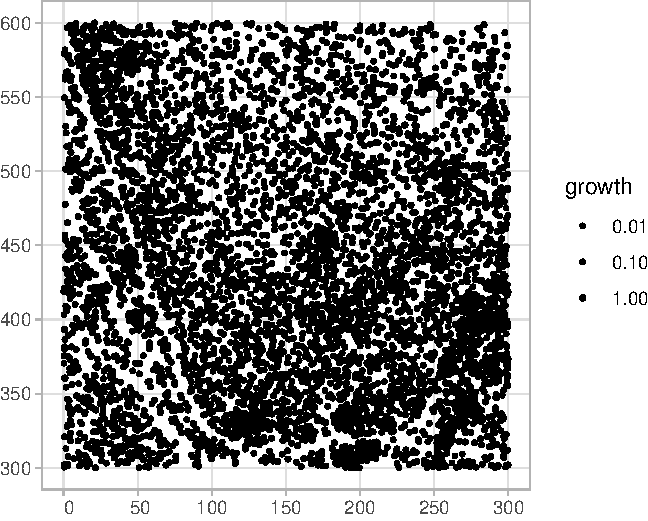
\includegraphics[width=0.66\linewidth]{Figures/scbi-trees-1} 

}

\caption{Compute growth of trees based on census data: Map with growth of all trees from a 9 ha subsection of the Smithsonian Conservation Biology Institute (SCBI) forest plot.}\label{fig:scbi-trees}
\end{figure}

\hypertarget{spatial-information}{%
\subsection{Step 2: Add spatial information}\label{spatial-information}}

The next step in our analysis sequence is to add spatial information to
our main \texttt{growth\_scbi} data frame. The first element of spatial
information we add is a ``buffer region'' to the periphery of the study
region. Since some of our model's explanatory variables are cumulative
(such as competitor basal area), we must ensure that all trees being
modeled are not biased to have different neighbor structures. This is of
concern for trees at the boundary of study regions, which will not have
the same number of neighbors as trees in the internal part of the study
region. In order to account for such edge effects, only trees that are
not part of this buffer region, i.e.~are part of the interior of the
study region, will have their growths modeled
\citet{waller_applied_2004}.

Our model of interspecific competition relies on a spatial definition of
who the competitor trees are for focal trees of interest: all trees
within a distance \texttt{comp\_dist} of a focal tree are considered its
competitors (assuming the same units as the \texttt{gx} and \texttt{gy}
location variables). In our case we set this value at 7.5m, a value
informed by \citet{canham_neighborhood_2004}
\citet{uriarte_spatially_2004} \citet{canham_neighborhood_2006}. Using
this value along with a manually constructed \texttt{sf} object
representation of the study region's boundary, we apply the
\texttt{add\_buffer\_variable()} to our \texttt{growth\_scbi} data frame
to add a \texttt{buffer} boolean variable: all trees who have
\texttt{buffer} set to \texttt{FALSE} will be our focal trees whose
growths are modeled, whereas those with \texttt{TRUE} will only be
considered as competitor trees whose growth will not be modeled.

\begin{Shaded}
\begin{Highlighting}[]
\CommentTok{# Define buffer region using competitive distance range}
\NormalTok{comp_dist <-}\StringTok{ }\FloatTok{7.5}

\NormalTok{study_region_scbi <-}\StringTok{ }\KeywordTok{tibble}\NormalTok{(}
  \DataTypeTok{x =} \KeywordTok{c}\NormalTok{(}\DecValTok{0}\NormalTok{, }\DecValTok{300}\NormalTok{, }\DecValTok{300}\NormalTok{, }\DecValTok{0}\NormalTok{, }\DecValTok{0}\NormalTok{),}
  \DataTypeTok{y =} \KeywordTok{c}\NormalTok{(}\DecValTok{300}\NormalTok{, }\DecValTok{300}\NormalTok{, }\DecValTok{600}\NormalTok{, }\DecValTok{600}\NormalTok{, }\DecValTok{300}\NormalTok{)}
\NormalTok{) }\OperatorTok
\StringTok{  }\KeywordTok{sf_polygon}\NormalTok{()}

\NormalTok{growth_scbi <-}\StringTok{ }\NormalTok{growth_scbi }\OperatorTok
\StringTok{  }\KeywordTok{add_buffer_variable}\NormalTok{(}\DataTypeTok{size =}\NormalTok{ comp_dist, }\DataTypeTok{region =}\NormalTok{ study_region_scbi)}
\end{Highlighting}
\end{Shaded}

The second element of spatial information are blocks corresponding to
folds of a spatial cross-validation algorithm used to estimate
out-of-sample model error. Conventional cross-validation algorithms
assign observations to folds by randomly resampling individual
observations. However, an assumption that the observations are
independent underlies any cross-validation algorithm. In the case of
forest census data, observations exhibit spatial autocorrelation. We
therefore incorporate this spatial dependence into the cross-validation
algorithm by randomly resampling spatial blocks of trees
\citet{roberts_cross-validation_2017}
\citet{pohjankukka_estimating_2017}.

In the example below, we first manually define four folds that partition
the study region as an \texttt{sf} object. We then use the output of the
\texttt{spatialBlock()} function from the \texttt{blockCV} package to
associate each tree in \texttt{growth\_scbi} to the correct fold (saved
in the \texttt{foldID} variable) \citet{valavi_blockcv_2019}. \footnote{In
  the Appendix we present an example where the folds themselves are also
  created using the \texttt{spatialBlock()} function given a specified
  \texttt{cv\_block\_size}.}

\begin{Shaded}
\begin{Highlighting}[]
\CommentTok{# Manually define spatial blocks to act as folds}
\NormalTok{n_fold <-}\StringTok{ }\DecValTok{4}
\NormalTok{fold1 <-}\StringTok{ }\KeywordTok{rbind}\NormalTok{(}\KeywordTok{c}\NormalTok{(}\DecValTok{0}\NormalTok{, }\DecValTok{300}\NormalTok{), }\KeywordTok{c}\NormalTok{(}\DecValTok{150}\NormalTok{, }\DecValTok{300}\NormalTok{), }\KeywordTok{c}\NormalTok{(}\DecValTok{150}\NormalTok{, }\DecValTok{450}\NormalTok{), }\KeywordTok{c}\NormalTok{(}\DecValTok{0}\NormalTok{, }\DecValTok{450}\NormalTok{))}
\NormalTok{fold2 <-}\StringTok{ }\KeywordTok{rbind}\NormalTok{(}\KeywordTok{c}\NormalTok{(}\DecValTok{150}\NormalTok{, }\DecValTok{300}\NormalTok{), }\KeywordTok{c}\NormalTok{(}\DecValTok{300}\NormalTok{, }\DecValTok{300}\NormalTok{), }\KeywordTok{c}\NormalTok{(}\DecValTok{300}\NormalTok{, }\DecValTok{450}\NormalTok{), }\KeywordTok{c}\NormalTok{(}\DecValTok{150}\NormalTok{, }\DecValTok{450}\NormalTok{))}
\NormalTok{fold3 <-}\StringTok{ }\KeywordTok{rbind}\NormalTok{(}\KeywordTok{c}\NormalTok{(}\DecValTok{0}\NormalTok{, }\DecValTok{450}\NormalTok{), }\KeywordTok{c}\NormalTok{(}\DecValTok{150}\NormalTok{, }\DecValTok{450}\NormalTok{), }\KeywordTok{c}\NormalTok{(}\DecValTok{150}\NormalTok{, }\DecValTok{600}\NormalTok{), }\KeywordTok{c}\NormalTok{(}\DecValTok{0}\NormalTok{, }\DecValTok{600}\NormalTok{))}
\NormalTok{fold4 <-}\StringTok{ }\KeywordTok{rbind}\NormalTok{(}\KeywordTok{c}\NormalTok{(}\DecValTok{150}\NormalTok{, }\DecValTok{450}\NormalTok{), }\KeywordTok{c}\NormalTok{(}\DecValTok{300}\NormalTok{, }\DecValTok{450}\NormalTok{), }\KeywordTok{c}\NormalTok{(}\DecValTok{300}\NormalTok{, }\DecValTok{600}\NormalTok{), }\KeywordTok{c}\NormalTok{(}\DecValTok{150}\NormalTok{, }\DecValTok{600}\NormalTok{))}

\NormalTok{blocks_scbi <-}\StringTok{ }\KeywordTok{bind_rows}\NormalTok{(}
  \KeywordTok{sf_polygon}\NormalTok{(fold1), }\KeywordTok{sf_polygon}\NormalTok{(fold2), }\KeywordTok{sf_polygon}\NormalTok{(fold3), }\KeywordTok{sf_polygon}\NormalTok{(fold4)}
\NormalTok{) }\OperatorTok
\StringTok{  }\KeywordTok{mutate}\NormalTok{(}\DataTypeTok{folds =} \KeywordTok{c}\NormalTok{(}\DecValTok{1}\OperatorTok{:}\NormalTok{n_fold) }\OperatorTok\StringTok{ }\KeywordTok{factor}\NormalTok{())}

\CommentTok{# Associate each observation to a fold}
\NormalTok{SpatialBlock_scbi <-}\StringTok{ }\KeywordTok{spatialBlock}\NormalTok{(}
  \DataTypeTok{speciesData =}\NormalTok{ growth_scbi, }\DataTypeTok{k =}\NormalTok{ n_fold, }\DataTypeTok{selection =} \StringTok{"systematic"}\NormalTok{, }
  \DataTypeTok{blocks =}\NormalTok{ blocks_scbi, }\DataTypeTok{showBlocks =} \OtherTok{FALSE}\NormalTok{, }\DataTypeTok{verbose =} \OtherTok{FALSE}
\NormalTok{)}

\NormalTok{growth_scbi <-}\StringTok{ }\NormalTok{growth_scbi }\OperatorTok
\StringTok{  }\KeywordTok{mutate}\NormalTok{(}\DataTypeTok{foldID =}\NormalTok{ SpatialBlock_scbi}\OperatorTok{$}\NormalTok{foldID }\OperatorTok\StringTok{ }\KeywordTok{factor}\NormalTok{())}
\end{Highlighting}
\end{Shaded}

Figure \ref{fig:scbi-spatial-information} illustrates the net effect of
adding these two elements of information to the \texttt{growth\_scbi}
data frame. The location of each tree is marked with an integer
indicating which fold it belongs to, where the folds are marked with
solid lines. The color of each digit indicates whether the tree is part
of the buffer region (and thus will only be considered as a competitor
tree in our model) or is part of the interior of the study region (and
thus is a focal tree whose growth is of modeled interest).

\begin{Shaded}
\begin{Highlighting}[]
\KeywordTok{ggplot}\NormalTok{() }\OperatorTok{+}
\StringTok{  }\KeywordTok{geom_sf}\NormalTok{(}\DataTypeTok{data =}\NormalTok{ blocks_scbi, }\DataTypeTok{fill =} \StringTok{"transparent"}\NormalTok{, }\DataTypeTok{linetype =} \StringTok{"dashed"}\NormalTok{) }\OperatorTok{+}
\StringTok{  }\KeywordTok{geom_sf_text}\NormalTok{(}\DataTypeTok{data =}\NormalTok{ growth_scbi }\OperatorTok\StringTok{ }\KeywordTok{sample_n}\NormalTok{(}\DecValTok{1000}\NormalTok{), }\KeywordTok{aes}\NormalTok{(}\DataTypeTok{label =}\NormalTok{ foldID, }\DataTypeTok{col =}\NormalTok{ buffer))}
\end{Highlighting}
\end{Shaded}

\begin{figure}

{\centering 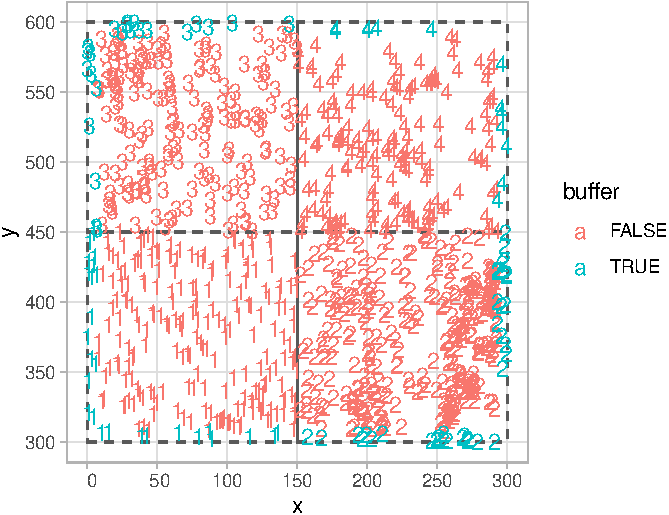
\includegraphics[width=0.66\linewidth]{Figures/scbi-spatial-information-1} 

}

\caption{Add spatial information: Buffer region and spatial cross-validation blocks (1 through 4). All trees in the interior of the study region (i.e. not part of buffer) will be the focal trees whose growth will be modeled.}\label{fig:scbi-spatial-information}
\end{figure}

\hypertarget{focal-vs-comp}{%
\subsection{Step 3: Identify all focal and corresponding competitor
trees}\label{focal-vs-comp}}

The next step in our analysis sequence is to identify all focal trees
and their corresponding competitor trees. The
\texttt{create\_focal\_vs\_comp()} functions performs these tasks and
returns a new data frame of type \texttt{sf}. On top of the previous
arguments \texttt{comp\_dist} defining the competition neighborhood and
\texttt{id} indicating which variable uniquely identifies each
tree-stem, this function also requires an \texttt{sf} object
representation of the spatial cross-validation blocks/folds; in our
case, this was manually encoded in the \texttt{blocks\_scbi} in Section
\ref{spatial-information} while in our Appendix we present an example
where this was performed using \texttt{spatialBlock()} from the
\texttt{blockCV} package. We present the resulting data frame below with
the \texttt{foldID} variable omitted for compactness of presentation.

\begin{Shaded}
\begin{Highlighting}[]
\CommentTok{# }\AlertTok{TODO}\CommentTok{: Below reconcile the number of rows as they off by one from growth_scbi %>% }
\CommentTok{# filter(!is.na(growth) & !buffer). Perhaps by removing NA's in the growth_scbi stage?}
\NormalTok{focal_vs_comp_scbi <-}\StringTok{ }\NormalTok{growth_scbi }\OperatorTok
\StringTok{  }\KeywordTok{create_focal_vs_comp}\NormalTok{(comp_dist, }\DataTypeTok{cv_grid_sf =}\NormalTok{ blocks_scbi, }\DataTypeTok{id =} \StringTok{"stemID"}\NormalTok{)}
\NormalTok{focal_vs_comp_scbi }\OperatorTok\StringTok{ }
\StringTok{  }\KeywordTok{select}\NormalTok{(}\OperatorTok{-}\NormalTok{foldID)}
\CommentTok{## # A tibble: 6,296 x 6}
\CommentTok{##    focal_ID focal_sp   dbh     geometry  growth comp             }
\CommentTok{##       <dbl> <fct>    <dbl>      <POINT>   <dbl> <list>           }
\CommentTok{##  1        4 nysy     13.6  (14.2 428.5)  0.103  <tibble [20 x 4]>}
\CommentTok{##  2        5 havi      8.8   (9.4 436.4)  0.150  <tibble [32 x 4]>}
\CommentTok{##  3       79 tiam     47.7    (40 381.1) -0.161  <tibble [20 x 4]>}
\CommentTok{##  4       80 caca      5.15 (38.7 421.7)  0.253  <tibble [12 x 4]>}
\CommentTok{##  5       96 libe      2.3      (60 310)  0.262  <tibble [14 x 4]>}
\CommentTok{##  6      101 litu     65.4  (47.1 567.3)  0.552  <tibble [19 x 4]>}
\CommentTok{##  7      102 astr      1.99 (40.8 575.5)  0.0954 <tibble [44 x 4]>}
\CommentTok{##  8      126 cato     37.4  (60.6 400.2)  0.165  <tibble [16 x 4]>}
\CommentTok{##  9      127 caca      8.72 (72.7 514.1)  0.0370 <tibble [14 x 4]>}
\CommentTok{## 10      139 astr      1.71 (96.7 315.1)  0.0549 <tibble [48 x 4]>}
\CommentTok{## # ... with 6,286 more rows}
\end{Highlighting}
\end{Shaded}

The resulting data frame \texttt{focal\_vs\_comp\_scbi} has 6296 rows,
representing the subset of the 7954 trees in \texttt{growth\_scbi} that
will be considered as focal trees. Two new variables \texttt{focal\_ID}
and \texttt{focal\_sp} relate to tree-stem identification and species
information. Most notably however is a new variable \texttt{comp} which
contains information on all competitor trees for a given focal tree,
saved in \texttt{tidyr} package list-column format
\citet{tidyr_package}. For example, we drill-down on the tree with
\texttt{focal\_ID} 4, which has 20 competitor trees each described by 4
variables as indicated by the fact that \texttt{comp} is a
\texttt{\textless{}tibble\ {[}20\ ×\ 4{]}\textgreater{}}.

\begin{Shaded}
\begin{Highlighting}[]
\NormalTok{focal_vs_comp_scbi }\OperatorTok\StringTok{ }
\StringTok{  }\KeywordTok{filter}\NormalTok{(focal_ID }\OperatorTok{==}\StringTok{ }\DecValTok{4}\NormalTok{) }\OperatorTok\StringTok{ }
\StringTok{  }\KeywordTok{select}\NormalTok{(focal_ID, dbh, comp)}
\CommentTok{## # A tibble: 1 x 3}
\CommentTok{##   focal_ID   dbh comp             }
\CommentTok{##      <dbl> <dbl> <list>           }
\CommentTok{## 1        4  13.6 <tibble [20 x 4]>}
\end{Highlighting}
\end{Shaded}

The spatial distribution of these trees is visualized in Figure
\ref{fig:scbi-focal-vs-comp-map}: the dashed circle extends 7.5 m away
from the focal tree while all 20 competitor trees are within this
circle.

\begin{figure}

{\centering 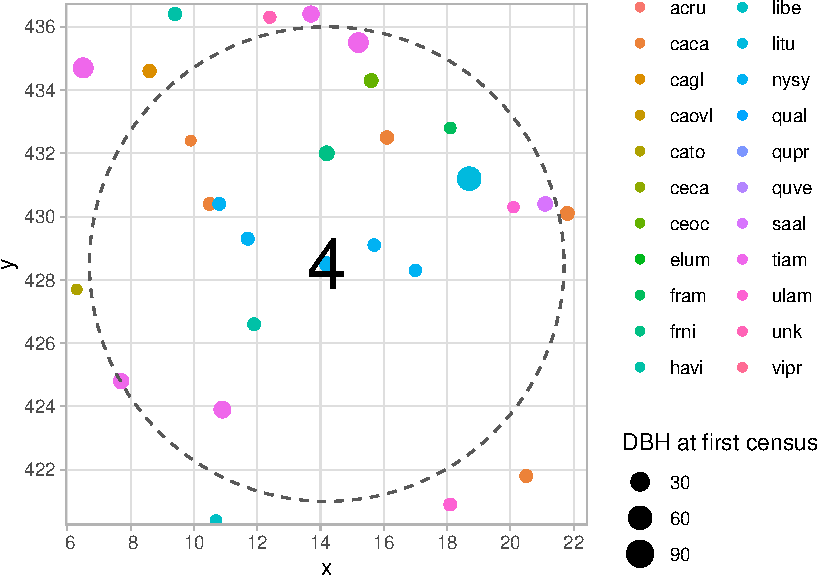
\includegraphics[width=0.66\linewidth]{Figures/scbi-focal-vs-comp-map-1} 

}

\caption{Identify all focal and corresponding competitor trees: All 20 competitor trees of focal tree 4.}\label{fig:scbi-focal-vs-comp-map}
\end{figure}

Using the \texttt{unnest()} function from the \texttt{tidyr} package, we
can flatten list-column into regular columns. We observe that for the
same focal tree, we have information on all 20 competitor trees whose
\texttt{dist} distance to the focal tree is \(\leq\) 7.5: their unique
tree-stem ID number, their species, and their basal area (in m\(^2\))
calculated as \(\frac{\pi \times (\text{DBH/2})^2}{10000}\) where
\(DBH\) is the value from the earlier of the two censuses in cm. Saving
our focal versus competitor information in list-column minimizes
redundancy since we do not repeat information on the focal tree 20
times.

\begin{Shaded}
\begin{Highlighting}[]
\NormalTok{focal_vs_comp_scbi }\OperatorTok\StringTok{ }
\StringTok{  }\KeywordTok{filter}\NormalTok{(focal_ID }\OperatorTok{==}\StringTok{ }\DecValTok{4}\NormalTok{) }\OperatorTok\StringTok{ }
\StringTok{  }\KeywordTok{select}\NormalTok{(focal_ID, dbh, comp) }\OperatorTok\StringTok{ }
\StringTok{  }\KeywordTok{unnest}\NormalTok{(}\DataTypeTok{cols =} \StringTok{"comp"}\NormalTok{)}
\end{Highlighting}
\end{Shaded}

\begin{verbatim}
## # A tibble: 20 x 6
##   focal_ID   dbh comp_ID  dist comp_sp comp_basal_area
##      <dbl> <dbl>   <dbl> <dbl> <fct>             <dbl>
## 1        4  13.6    1836  7.48 tiam            0.0176 
## 2        4  13.6    1847  2.81 nysy            0.00332
## 3        4  13.6    1848  1.62 nysy            0.00396
## 4        4  13.6    1849  2.62 nysy            0.00535
## 5        4  13.6    1850  2.98 havi            0.00472
## # ... with 15 more rows
\end{verbatim}

\hypertarget{model-fit-predict}{%
\subsection{Step 4: Fit model}\label{model-fit-predict}}

Now that we've identified all focal and corresponding competitor trees
and saved this information in a data frame of type
\texttt{focal\_vs\_comp}, the final step in our analysis sequence is to
fit a model for the growth of all focal trees. Currently the
\texttt{forestecology} package can only fit the competition Bayesian
linear regression model outlined in Section \ref{competition-model}
using the \texttt{comp\_bayes\_lm()} function. However, any model
implemented in a function that similarly takes an input data frame of
type \texttt{focal\_vs\_comp} as an argument can be easily swapped in.
For our specific competition Bayesian linear regression model, we also
specify prior distributions on all parameters of interest (here chosen
to be the defaults as specified in \texttt{?comp\_bayes\_lm}).

\begin{Shaded}
\begin{Highlighting}[]
\CommentTok{# }\AlertTok{TODO}\CommentTok{: Add information about default priors in ?comp_bayes_lm()}
\NormalTok{comp_bayes_lm_scbi <-}\StringTok{ }\NormalTok{focal_vs_comp_scbi }\OperatorTok
\StringTok{  }\KeywordTok{comp_bayes_lm}\NormalTok{(}\DataTypeTok{prior_param =} \OtherTok{NULL}\NormalTok{)}
\end{Highlighting}
\end{Shaded}

The returned \texttt{comp\_bayes\_lm\_scbi} output is an object of S3
class type \texttt{comp\_bayes\_lm} which contains the posterior values
of all parameters in our competition Bayesian linear regression. This
class of object includes generic methods implemented for
\texttt{print()}, \texttt{predict()}, and \texttt{ggplot2::autoplot()}.
First the generic for \texttt{print()} displays the names of all prior
\& posterior parameters along with the model formula:

\begin{Shaded}
\begin{Highlighting}[]
\NormalTok{comp_bayes_lm_scbi}
\CommentTok{## Bayesian linear regression model parameters with a multivariate Normal likelihood. See ?comp_bayes_lm for details:}
\CommentTok{## }
\CommentTok{##   parameter_type           prior posterior}
\CommentTok{## 1 Inverse-Gamma on sigma^2 a_0   a_star   }
\CommentTok{## 2 Inverse-Gamma on sigma^2 b_0   b_star   }
\CommentTok{## 3 Multivariate t on beta   mu_0  mu_star  }
\CommentTok{## 4 Multivariate t on beta   V_0   V_star   }
\CommentTok{## }
\CommentTok{## Model formula:}
\CommentTok{## growth ~ sp + dbh + dbh * sp + acne * sp + acpl * sp + acru * sp + acsp * sp + aial * sp + amar * sp + astr * sp + beth * sp + caca * sp + caco * sp + cade * sp + cagl * sp + caovl * sp + casp * sp + cato * sp + ceca * sp + ceoc * sp + chvi * sp + coal * sp + coam * sp + cofl * sp + crpr * sp + crsp * sp + divi * sp + elum * sp + eual * sp + fagr * sp + fram * sp + frni * sp + frpe * sp + frsp * sp + havi * sp + ilve * sp + juci * sp + juni * sp + juvi * sp + libe * sp + litu * sp + loma * sp + nysy * sp + pato * sp + pipu * sp + pist * sp + pivi * sp + ploc * sp + prav * sp + prpe * sp + prse * sp + prsp * sp + qual * sp + quco * sp + qufa * sp + qumi * sp + qupr * sp + quru * sp + qusp * sp + quve * sp + rhpe * sp + romu * sp + rops * sp + rual * sp + rupe * sp + ruph * sp + saal * sp + saca * sp + tiam * sp + ulam * sp + ulru * sp + ulsp * sp + unk * sp + viac * sp + vipr * sp + vire * sp}
\end{Highlighting}
\end{Shaded}

Next, the generic for \texttt{predict()} takes as inputs the posterior
parameter values in \texttt{comp\_bayes\_lm\_scbi} and the predictor
variables in \texttt{newdata} and outputs a vector of fitted/predicted
values \(\widehat{y}\) of the DBH for each focal tree computed from the
posterior predictive distribution.

\begin{Shaded}
\begin{Highlighting}[]
\NormalTok{focal_vs_comp_scbi <-}\StringTok{ }\NormalTok{focal_vs_comp_scbi }\OperatorTok
\StringTok{  }\KeywordTok{mutate}\NormalTok{(}\DataTypeTok{growth_hat =} \KeywordTok{predict}\NormalTok{(comp_bayes_lm_scbi, }\DataTypeTok{newdata =}\NormalTok{ focal_vs_comp_scbi))}
\end{Highlighting}
\end{Shaded}

\begin{Shaded}
\begin{Highlighting}[]
\NormalTok{focal_vs_comp_scbi}
\CommentTok{## # A tibble: 6,296 x 8}
\CommentTok{##    focal_ID focal_sp   dbh foldID                  geometry  growth}
\CommentTok{##       <dbl> <fct>    <dbl> <fct>                    <POINT>   <dbl>}
\CommentTok{##  1        4 nysy     13.6  1                   (14.2 428.5)  0.103 }
\CommentTok{##  2        5 havi      8.8  1                    (9.4 436.4)  0.150 }
\CommentTok{##  3       79 tiam     47.7  1                     (40 381.1) -0.161 }
\CommentTok{##  4       80 caca      5.15 1                   (38.7 421.7)  0.253 }
\CommentTok{##  5       96 libe      2.3  1                       (60 310)  0.262 }
\CommentTok{##  6      101 litu     65.4  3                   (47.1 567.3)  0.552 }
\CommentTok{##  7      102 astr      1.99 3                   (40.8 575.5)  0.0954}
\CommentTok{##  8      126 cato     37.4  1                   (60.6 400.2)  0.165 }
\CommentTok{##  9      127 caca      8.72 3                   (72.7 514.1)  0.0370}
\CommentTok{## 10      139 astr      1.71 1                   (96.7 315.1)  0.0549}
\CommentTok{## # ... with 6,286 more rows, and 2 more variables: comp <list>,}
\CommentTok{## #   growth_hat <dbl>}
\end{Highlighting}
\end{Shaded}

We then compare the observed and fitted/predicted growths to compute the
root mean squared error (RMSE) of our model fit.

\begin{Shaded}
\begin{Highlighting}[]
\NormalTok{model_rmse <-}\StringTok{ }\NormalTok{focal_vs_comp_scbi }\OperatorTok
\StringTok{  }\KeywordTok{rmse}\NormalTok{(}\DataTypeTok{truth =}\NormalTok{ growth, }\DataTypeTok{estimate =}\NormalTok{ growth_hat) }\OperatorTok
\StringTok{  }\KeywordTok{pull}\NormalTok{(.estimate)}
\NormalTok{model_rmse}
\CommentTok{## [1] 0.1281398}
\end{Highlighting}
\end{Shaded}

Lastly, the generic for \texttt{ggplot2::autoplot()} allows us to plot
the posterior distribution of all parameters in Figure
\ref{fig:scbi-posterior-viz} (for compactness we only show posteriors
for 3 species).

\begin{Shaded}
\begin{Highlighting}[]
\CommentTok{# Plot posteriors for only a subset of species}
\NormalTok{sp_to_plot <-}\StringTok{ }\KeywordTok{c}\NormalTok{(}\StringTok{"litu"}\NormalTok{, }\StringTok{"quru"}\NormalTok{, }\StringTok{"cagl"}\NormalTok{)}

\NormalTok{plot1 <-}\StringTok{ }\KeywordTok{autoplot}\NormalTok{(comp_bayes_lm_scbi, }\DataTypeTok{type =} \StringTok{"intercepts"}\NormalTok{, }\DataTypeTok{sp_to_plot =}\NormalTok{ sp_to_plot)}
\NormalTok{plot2 <-}\StringTok{ }\KeywordTok{autoplot}\NormalTok{(comp_bayes_lm_scbi, }\DataTypeTok{type =} \StringTok{"dbh_slopes"}\NormalTok{, }\DataTypeTok{sp_to_plot =}\NormalTok{ sp_to_plot)}
\NormalTok{plot3 <-}\StringTok{ }\KeywordTok{autoplot}\NormalTok{(comp_bayes_lm_scbi, }\DataTypeTok{type =} \StringTok{"competition"}\NormalTok{, }\DataTypeTok{sp_to_plot =}\NormalTok{ sp_to_plot)}

\CommentTok{# Combine plots using patchwork}
\NormalTok{(plot1 }\OperatorTok{|}\StringTok{ }\NormalTok{plot2) }\OperatorTok{/}\StringTok{ }\NormalTok{plot3}
\end{Highlighting}
\end{Shaded}

\begin{figure}

{\centering 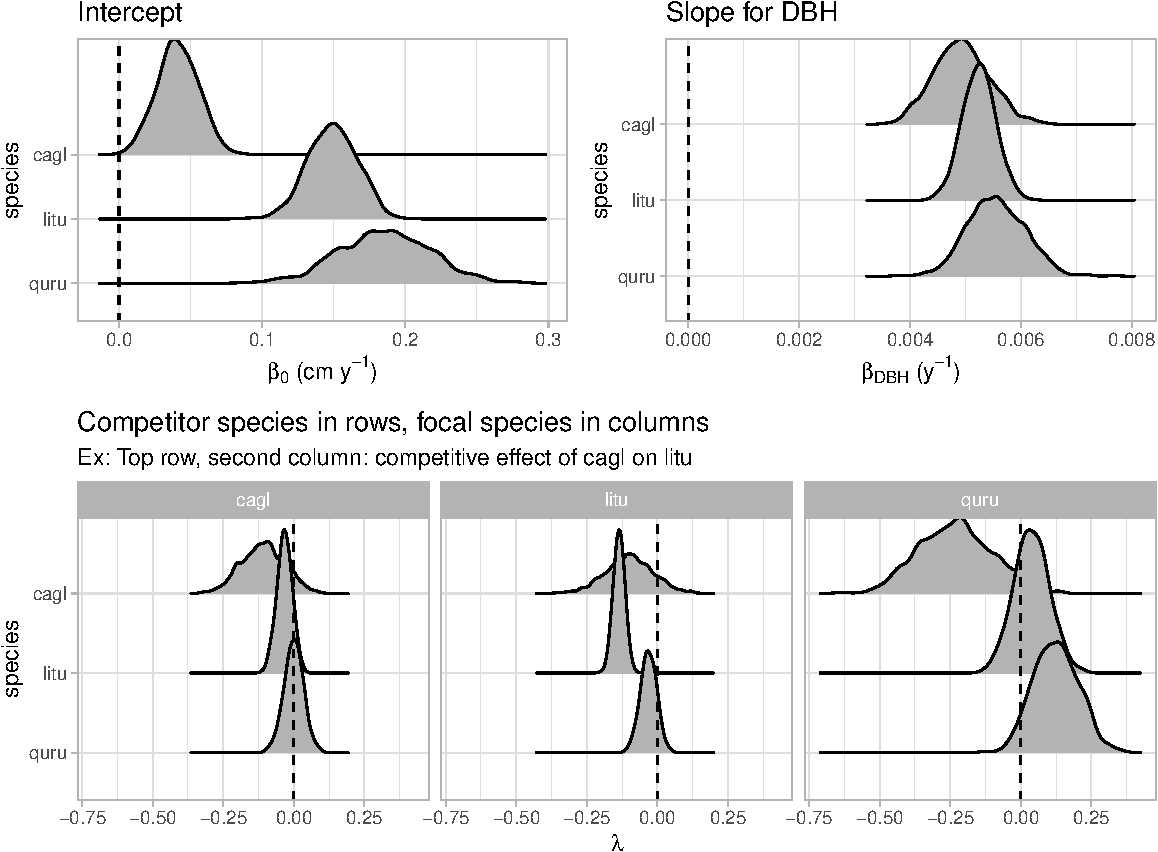
\includegraphics[width=1\linewidth]{Figures/scbi-posterior-viz-1} 

}

\caption{Fit model: Posterior distributions of all parameters for three species.}\label{fig:scbi-posterior-viz}
\end{figure}

TODO: Discuss meaning of results.

\hypertarget{evaluate-the-effect-of-competitor-species-identity-using-permutation-tests}{%
\subsection{Evaluate the effect of competitor species identity using
permutation
tests}\label{evaluate-the-effect-of-competitor-species-identity-using-permutation-tests}}

In order to evaluate the effect of competitor species identity, we use
the four steps of our analysis sequence answer along with a permutation
test: Under a null hypothesis where competitor species identity does not
matter, we can permute/shuffle this variable within each focal tree,
compute the RMSE (the test statistic of interest), repeat this process
several times to construct a null distribution of the RMSE, and compare
it to the observed RMSE to assess significance. Going back to our
example in Section \ref{focal-vs-comp} of focal tree with
\texttt{focal\_ID} 4 and its 20 competitors, the permutation test
randomly resamples the \texttt{comp\_sp} variable with replacement,
leaving all other variables intact. The resampling with replacement is
nested within each focal tree in order to preserve the neighborhood
structure of our competition model. To run the permutation test, we use
the same\texttt{comp\_bayes\_lm()} function as in Section
\ref{model-fit-predict}, but with a \texttt{run\_shuffle\ =\ TRUE}
argument.

\begin{Shaded}
\begin{Highlighting}[]
\NormalTok{comp_bayes_lm_scbi_shuffle <-}\StringTok{ }\NormalTok{focal_vs_comp_scbi }\OperatorTok
\StringTok{  }\KeywordTok{comp_bayes_lm}\NormalTok{(}\DataTypeTok{prior_param =} \OtherTok{NULL}\NormalTok{, }\DataTypeTok{run_shuffle =} \OtherTok{TRUE}\NormalTok{)}

\NormalTok{focal_vs_comp_scbi <-}\StringTok{ }\NormalTok{focal_vs_comp_scbi }\OperatorTok
\StringTok{  }\KeywordTok{mutate}\NormalTok{(}\DataTypeTok{growth_hat_shuffle =} \KeywordTok{predict}\NormalTok{(comp_bayes_lm_scbi_shuffle, }\DataTypeTok{newdata =}\NormalTok{ focal_vs_comp_scbi))}

\NormalTok{model_rmse_shuffle <-}\StringTok{ }\NormalTok{focal_vs_comp_scbi }\OperatorTok
\StringTok{  }\KeywordTok{rmse}\NormalTok{(}\DataTypeTok{truth =}\NormalTok{ growth, }\DataTypeTok{estimate =}\NormalTok{ growth_hat_shuffle) }\OperatorTok
\StringTok{  }\KeywordTok{pull}\NormalTok{(.estimate)}
\NormalTok{model_rmse_shuffle}
\CommentTok{## [1] 0.131083}
\end{Highlighting}
\end{Shaded}

The resulting RMSE of 0.131083 based on the permutation test is larger
than the earlier RMSE of 0.1281398, suggesting that models that do
incorporate competitor species identity better fit the data. We conduct
a fuller simulation in Section below.

\hypertarget{spatial-cross-validation}{%
\subsection{Evaluate model performance using spatial
cross-validation}\label{spatial-cross-validation}}

We answer the second of our two questions: how can we obtain an accurate
estimate of model performance/error? The model fits and predictions in
Section \ref{model-fit-predict} all suffer from a common failing: they
use the same data to both fit the model and to assess the model's
performance using the RMSE. As argued by
\citet{roberts_cross-validation_2017}, this can lead to overly
optimistic assessments of model quality as the models can be overfit, in
particular in situations where spatial-autocorrelation is present. To
mitigate the effects of such overfitting, we use a spatially block
cross-validation algorithm.

To this end, we use the \texttt{foldID} variable defined in Section
\ref{spatial-information} whereby all focal trees are assigned to one of
4 spatially contiguous blocks that act as folds in our cross-validation
routine. Figure \ref{fig:scbi-spatial-cross-validation-schematic}
presents a schematic illustrating this scheme for fold 1 (bottom-left)
as the test set and folds 2, 3, and 4 as the training sets. We fit the
model to all focal trees in the training set, apply the model to all
focal trees in the test set to compute fitted/predicted values, and
compute the RMSE of the observed versus predicted growths. We repeat
this procedure 3 more times with each of the three remaining folds
acting as the test set and then average all four resulting RMSE's.
Furthermore, in order to maintain spatial independence between the test
and training set, a buffer that extend outwards from the boundary of the
test set is computed; all trees falling within this buffer are excluded
from the training set.

\begin{figure}

{\centering 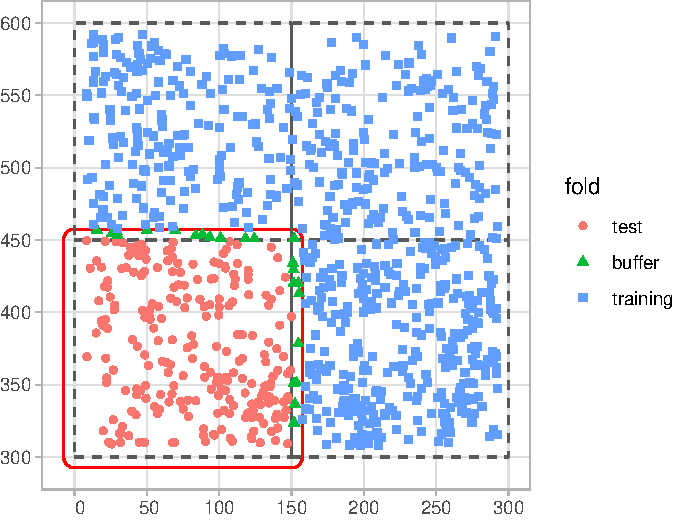
\includegraphics[width=0.66\linewidth]{Figures/scbi-spatial-cross-validation-schematic-1} 

}

\caption{Schematic of spatial cross-validation: Using the k = 1 fold as the test set, assigning each focal tree to training set, test set, and buffer.}\label{fig:scbi-spatial-cross-validation-schematic}
\end{figure}

This algorithm is implemented in the \texttt{run\_cv()} function, which
is a wrapper function to the \texttt{comp\_bayes\_lm()} function that
fits the model and the \texttt{predict()} generic that returns
fitted/predicted values. We compare these values to the observed growth
values to again compute our RMSE.

\begin{Shaded}
\begin{Highlighting}[]
\NormalTok{focal_vs_comp_scbi <-}\StringTok{ }\NormalTok{focal_vs_comp_scbi }\OperatorTok
\StringTok{  }\KeywordTok{run_cv}\NormalTok{(}\DataTypeTok{comp_dist =}\NormalTok{ comp_dist, }\DataTypeTok{cv_grid =}\NormalTok{ blocks_scbi)}
\end{Highlighting}
\end{Shaded}

\begin{Shaded}
\begin{Highlighting}[]
\NormalTok{model_rmse_cv <-}\StringTok{ }\NormalTok{focal_vs_comp_scbi }\OperatorTok
\StringTok{  }\KeywordTok{rmse}\NormalTok{(}\DataTypeTok{truth =}\NormalTok{ growth, }\DataTypeTok{estimate =}\NormalTok{ growth_hat) }\OperatorTok
\StringTok{  }\KeywordTok{pull}\NormalTok{(.estimate)}
\NormalTok{model_rmse_cv}
\CommentTok{## [1] 0.1402209}
\end{Highlighting}
\end{Shaded}

The resulting RMSE of 0.1402209 computed using cross-validation is
larger than the earlier RMSE of 0.1281398, suggesting that models that
do not take the inherent spatial autocorrelation of the data into
account generate error estimates that are overly optimistic; in our case
RMSE's that are too low.

\hypertarget{discussion}{%
\section{Discussion}\label{discussion}}

\begin{itemize}
\tightlist
\item
  Run full simulation on SCBI data
\item
  run time considerations
\end{itemize}

\hypertarget{acknowledgments}{%
\section{Acknowledgments}\label{acknowledgments}}

Sophie Li for her feedback on package interface.

\bibliographystyle{agsm}
\bibliography{paper.bib}

\end{document}
